\section{Аналитический раздел}

\subsection{Постановка задачи}\label{sec:task}
В соответствии с заданием на курсовую работу необходимо разработать межсетевой экран, осуществляющий контроль проходящего сетевого трафика, в виде загружаемого модуля.

Для достижения поставленной цели необходимо решить следующие задачи:
\begin{enumerate}
	\item ознакомиться с основными принципами работы отдельных узлов распределённой системы и межсетевых экранов;
	
	\item ознакомиться со способом перехвата поступающих на хост пакетов;
	
	\item выбрать тип устройства для перехвата входящих и исходящих пакетов;
	
	\item разработать формат задания пользователем правил фильтрации пакетов и изменения видимости модуля в системе;
	
	\item реализовать межсетевой экран. \newline
\end{enumerate}

\subsection{Анализ процесса передачи информации}
В распределённых системах информация передаётся в виде пакетов по протоколам. Передаваемые данные подвергаются процессам инкапсуляции и декапсуляции, в процессе которых каждый пакет проходит все уровни модели OSI (таблица \ref{osi_table}) \cite{net}.

\begin{table}[h]
	\begin{center}
		\caption{Модель OSI}
		\label{osi_table}
		\begin{tabular}{| p{1cm} | p{7cm} |}
			\hline
			\textbf{№} 	& \textbf{Название} \\
			\hline
			7 		& Прикладной уровень\\ 
			\hline
			6 		& Уровень представления  \\ 
			\hline
			5 		& Сеансовый уровень \\ 
			\hline
			4 		& Транспортный уровень \\ 
			\hline
			3 		& Сетевой уровень \\ 
			\hline
			2 		& Канальный уровень \\ 
			\hline
			1 		& Физический уровень \\ 
			\hline
		\end{tabular}
	\end{center}
\end{table} 

\newpage

Широко распространённым средством перехвата и анализа входящих и исходящих пакетов принято называть межсетевым экраном. Он позволяет защищать как отдельный хост (рисунок \ref{fig1:image}), так и крупную сеть, в таком случае применяются аппаратно-программные комплексы. 

\begin{figure}[h]
	\centering
	\begin{center}
		{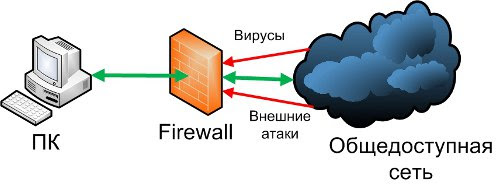
\includegraphics[scale=0.5]{img/firewall.jpg}}
		\caption{Принцип работы межсетевого экрана}
		\label{fig1:image}
	\end{center}
\end{figure}

Фильтрация пакетов происходит на пакетном уровне (уровни 3 и 4 модели OSI \cite{fw}), и при их обработке учитывается информация об IP-адресе источника/ назначения, номере порта источника/назначения и протоколе. \newline

\subsection{Загружаемые модули ядра}
Для того, чтобы добавить новые функции в ядро Linux, нужно либо перекомпилировать его (что небезопасно), либо воспользоваться загружаемым модулем ядра \cite{os}. 

После загрузки модуля он становится частью операционной системы и ему доступны все структуры и функции ядра. Когда функциональность, предоставляемая модулем, больше не требуется, то он может быть выгружен.

Модули загружаются и выгружаются с помощью специальных команд, приведённых в Листинге \ref{lst:module}.

\begin{lstlisting}[caption = {Команды для загрузки и выгрузки загружаемого модуля ядра}, label=lst:module]
insmod <имя модуля.ko>		// загрузить модуль в ядро
rmmod <имя модуля>			// выгрузить модуль из ядра
\end{lstlisting}

Загружаемый модуль ядра должен иметь определённую структуру. Обязательной частью любого загружаемого модуля являются:
\begin{itemize}
	\item функция загрузки (инициализации) модуля;
	
	\item функция выгрузки модуля; 
	
	\item макросы module\_init(init\_func), module\_exit(exit\_func);
	
	\item макрос MODULE\_LICENSE(char* license). \newline
\end{itemize}

\subsection{Анализ способа изменения видимости модуля}
Для того, чтобы заинтересованный пользователь не смог удалить средство контроля трафика, его необходимо сделать невидимым. Удаляя соответствующий элемент из связного списка модулей, он становится скрытым, и система не может предоставить информацию о данном загружаемом модуле.

Для взаимодействия со списком модулей необходимо использовать структуру \textbf{struct list\_head} и функции \textbf{list\_add}, \textbf{list\_del}. Перед удалением модуля из списка, следует сохранить его указатель для обеспечения возможности восстановить его видимость \cite{hide}.

Структура \textbf{struct module} (Листинг \ref{lst:struct_module}), описывающая модуль, предоставляет доступ к связному списку, где поле list -- его элемент.
\begin{lstlisting}[caption = {struct module}, label=lst:struct_module]
struct module
{
	enum module_state state;
	struct list_head list; /* Member of list of modules */
	char name[MODULE_NAME_LEN]; /* Unique handle for this module */
	...
};
\end{lstlisting}

\subsection{Анализ и выбор устройства для межсетевого экрана}
Как правило, для реализации межсетевых экранов используется \textbf{char} устройства \cite{2nd}, но поскольку разрабатываемый модуль предназначен только для одной задачи, рекомендуется использовать \textbf{misc} устройство \cite{2nd,misc}.

Для работы со специальными файлами в обоих случаях используется структура \textbf{struct file\_operations} (Листинг \ref{lst:file_op}). 
\begin{lstlisting}[caption = {struct file\_operations}, label=lst:file_op]
struct file_operations {
	struct module *owner;
	...
	ssize_t (*read) (struct file *, char __user *, size_t, loff_t *);
	ssize_t (*write) (struct file *, const char __user *, size_t, loff_t *);
	...
	int (*open) (struct inode *, struct file *);
	...
	int (*release) (struct inode *, struct file *);
	...
}
\end{lstlisting}

Указатель на неё хранится в структуре -- \textbf{struct miscdevice} (Листинг \ref{lst:misc}).
\begin{lstlisting}[caption = {struct miscdevice}, label=lst:misc]
struct miscdevice {
	int minor;
	const char *name;
	struct file_operations *fops;
	umode_t i_mode;
	struct miscdevice *next, *prev;
};
\end{lstlisting}

Старший номер misc устройства задан и равен 10, младший должен быть определён разработчиком, либо создан динамически, если указано значение MISC\_DYNAMIC\_MINOR в поле minor структуры struct miscdevice \cite{3d}. Для char устройства необходимо задавать и старший, и младший номера.

Функции для регистрации и удаления приведены в Листинге \ref{lst:misc_reg}. В процессе регистрации автоматически создаётся misc драйвер.

\begin{lstlisting}[caption = {Функции для регистрации и удаления misc устройства}, label=lst:misc_reg]
	int misc_register(struct miscdevice *misc);		// регистрация
	int misc_deregister(struct miscdevice *misc);	// удаление
\end{lstlisting}

\subsection{Анализ точек перехватов пакетов}
Существует 5 точек (рисунок \ref{fig2:image}), в которых пакет может быть перехвачен:
\begin{enumerate}
	\item NF\_INET\_PRE\_ROUTING – для всех входных пакетов;
	\item NF\_INET\_LOCAL\_IN – используется, чтобы перехватить пакеты, предназначенные для локального процесса;
	\item NF\_INET\_FORWARD – используется для пакетов, предназначенных для другого интерфейса;
	\item NF\_INET\_LOCAL\_OUT – для пакетов, которые создают локальные процессы;
	\item NF\_INET\_POST\_ROUTING – для пакетов, которые уже настроены для дальнейшего прохождения по сети к своему адресату и готовы покинуть текущий сетевой стек.
\end{enumerate}

\begin{figure}[h]
	\centering
	\begin{center}
		{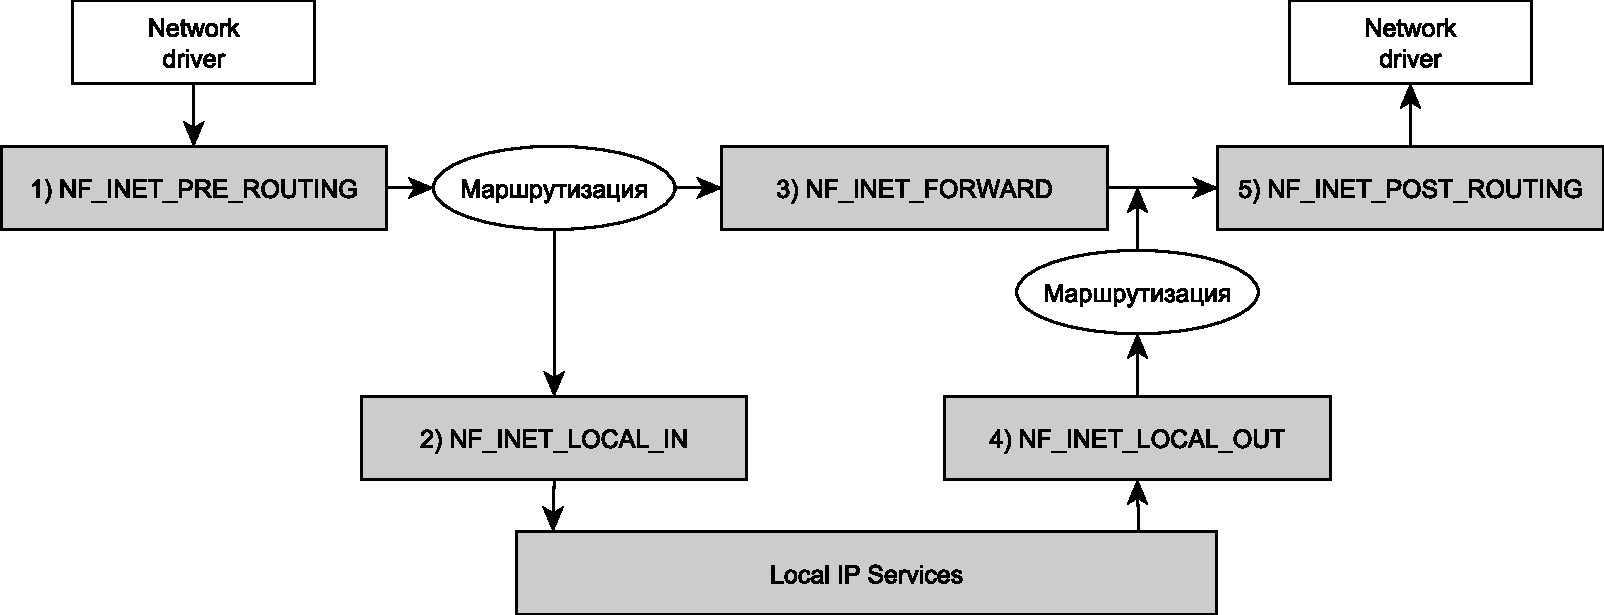
\includegraphics[scale=0.6]{img/packets.pdf}}
		\caption{Путь сетевого пакета}
		\label{fig2:image}
	\end{center}
\end{figure}

\newpage

На этих точках могут быть определены функции перехвата, которые называются \textbf{хук-функциями}. Для их определения необходима структура \textbf{struct nf\_hook\_ops} (Листинг \ref{lst:hook}).

\begin{lstlisting}[caption = {struct nf\_hook\_ops}, label=lst:hook]
struct nf_hook_ops {
	nf_hookfn			*hook;
	...
	u_int8_t			pf;
	unsigned int		hooknum;
	int					priority;
};
\end{lstlisting}

В структуре находятся поля:
\begin{itemize}
	\item \textbf{hook} -- функция, которая будет вызвана для обработки пакета, принимается решение отбросить или принять пакет;
	
	\item \textbf{pf} -- семейство протоколов;
	
	\item \textbf{hooknum} -- точка перехвата;
	
	\item \textbf{priority} -- приоритет. \\
\end{itemize}

Регистрация и удаление хуков осуществляется посредством вызова функций, которые представлены в Листинге \ref{lst:hook_reg}.

\begin{lstlisting}[caption = {Функции для регистрации и удаления хук-функций}, label=lst:hook_reg]
	// регистрация
	int nf_register_net_hook(struct net *net, const struct nf_hook_ops *ops);
	
	// удаление
	void nf_unregister_net_hook(struct net *net, const struct nf_hook_ops *ops);
\end{lstlisting}

\subsection*{Выводы}
\addcontentsline{toc}{subsection}{Выводы}
В результате сравнительного анализа для реализации межсетевого экрана было выбрано misc устройство, для которого автоматически создаётся соответствующий misc драйвер, ориентированный на выполнение конкретной задачи. Для перехвата входящих и исходящих сетевых пакетов предлагается использовать хук-функции, определённые на точках перехвата до маршрутизации и после неё. Для увеличения безопасности работы загружаемого модуля предлагается способ его сокрытия в системе посредством удаления соответствующего элемента из связного списка модулей.



 